\documentclass[13pt,a4paper]{article}
\usepackage[utf8]{inputenc}
\usepackage[T5]{fontenc}
\usepackage[fontsize=13pt]{scrextend}
\usepackage[left=3cm,right=2cm,top=2cm,bottom=2.5cm]{geometry}
\usepackage{mathptmx}
\usepackage{amsmath,amssymb}
\usepackage{graphicx}
\usepackage{float}
\usepackage{tikz}
\usetikzlibrary{calc,positioning,shapes.geometric,arrows.meta}
\usepackage{booktabs}
\usepackage{array}
\usepackage{tabularx}
\usepackage{longtable}
\usepackage{listings}
\usepackage{xcolor}
\usepackage{caption}
\usepackage{hyperref}
\usepackage{indentfirst}
\usepackage{titlesec}

\hypersetup{colorlinks=true,linkcolor=black,urlcolor=blue,citecolor=black}
\renewcommand{\baselinestretch}{1.25}
\setlength{\parindent}{1cm}
\setlength{\parskip}{6pt}
\setcounter{secnumdepth}{4}
\renewcommand{\contentsname}{MỤC LỤC}
\renewcommand{\listfigurename}{DANH MỤC HÌNH VẼ}
\renewcommand{\listtablename}{DANH MỤC BẢNG BIỂU}
\renewcommand{\figurename}{\bfseries Hình}
\renewcommand{\tablename}{\bfseries Bảng}
\renewcommand{\thefigure}{\thesection.\arabic{figure}}
\renewcommand{\thetable}{\thesection.\arabic{table}}
\captionsetup{labelsep=space,font=bf}
\renewcommand{\arraystretch}{1.25}
\setlength{\tabcolsep}{8pt}

\titleformat*{\section}{\fontsize{16pt}{18pt}\selectfont\bfseries\centering}
\titleformat*{\subsection}{\fontsize{14pt}{16pt}\selectfont\bfseries}
\titleformat*{\subsubsection}{\fontsize{13pt}{15pt}\selectfont\bfseries\itshape}
\titlespacing*{\section}{0pt}{0pt}{18pt}
\titlespacing*{\subsection}{0pt}{12pt}{4pt}
\titlespacing*{\subsubsection}{0pt}{10pt}{2pt}

\lstdefinestyle{verilogstyle}{
  language=Verilog,
  basicstyle=\ttfamily\small,
  keywordstyle=\color{blue}\bfseries,
  commentstyle=\color{gray}\itshape,
  stringstyle=\color{orange},
  numbers=left,
  numberstyle=\tiny,
  stepnumber=1,
  frame=single,
  breaklines=true,
  tabsize=2,
  columns=fullflexible
}

\newcommand{\placeholder}[2]{
\begin{figure}[H]
  \centering
  \fbox{\begin{minipage}[c][6cm][c]{0.86\textwidth}
    \centering \textbf{Chèn hình sau}\\[6pt]
    #2
  \end{minipage}}
  \caption{#1}
\end{figure}
}

\newcommand{\optionalimage}[3]{
\begin{figure}[H]
  \centering
  \IfFileExists{#1}{\includegraphics[width=0.86\textwidth]{#1}}{
    \fbox{\begin{minipage}[c][6cm][c]{0.86\textwidth}
      \centering \textbf{Chèn hình sau}\\[6pt]#3\\[4pt]\texttt{\detokenize{#1}}
    \end{minipage}}
  }
  \caption{#2}
\end{figure}
}

\begin{document}

\begin{titlepage}
\thispagestyle{empty}
\begin{tikzpicture}[overlay,remember picture]
\draw[line width=3pt] ($(current page.north west)+(3cm,-2cm)$) rectangle ($(current page.south east)+(-2cm,2.5cm)$);
\draw[line width=0.5pt] ($(current page.north west)+(3.1cm,-2.1cm)$) rectangle ($(current page.south east)+(-2.1cm,2.6cm)$);
\end{tikzpicture}
\begin{center}
ĐẠI HỌC BÁCH KHOA HÀ NỘI\\
\textbf{TRƯỜNG ĐIỆN - ĐIỆN TỬ}

\vspace{0.9cm}

\includegraphics[width=0.16\textwidth]{images/logoBK.png}

\vspace{1.0cm}
\textbf{\fontsize{22pt}{26pt}\selectfont BÁO CÁO MÔN HỌC}

\vspace{0.25cm}
\textbf{\fontsize{16pt}{20pt}\selectfont THIẾT KẾ TỔNG HỢP HỆ THỐNG SỐ}

\vspace{0.4cm}
\textbf{\fontsize{17pt}{21pt}\selectfont KHÓA SỐ BẢO MẬT\\
(DIGITAL SAFE LOCK) LƯU MẬT KHẨU VÀO SRAM}

\vspace{1.2cm}
\begin{tabular}{>{\bfseries}p{4cm}>{\raggedright\arraybackslash}p{10cm}}
Sinh viên thực hiện: & Nguyễn Văn Dương -- 20241713E\\
                     & Phạm Chí Dũng -- 20200106\\
GVHD: & TS. Nguyễn Hoàng Dũng\\
Đề tài: & \normalfont\begin{minipage}[t]{10cm}\raggedright Khóa số bảo mật (Digital Safe Lock) lưu mật khẩu vào SRAM\end{minipage}\\
\end{tabular}

\vfill
{\fontsize{14pt}{16pt}\selectfont Hà Nội, 07/2026}
\end{center}
\end{titlepage}

\pagenumbering{roman}
\section*{LỜI NÓI ĐẦU}
\addcontentsline{toc}{section}{LỜI NÓI ĐẦU}
Trong các hệ thống số, bài toán điều khiển truy cập bằng mật khẩu là một ví dụ phù hợp để kết hợp nhiều khối chức năng như nhận tín hiệu từ người dùng, chống dội nút nhấn, điều khiển tuần tự, lưu trữ dữ liệu và hiển thị trạng thái. Vì vậy, đề tài ``Khóa số bảo mật'' được lựa chọn nhằm vận dụng kiến thức của môn học Thiết kế tổng hợp hệ thống số vào một thiết kế RTL hoàn chỉnh trên FPGA.

Mục tiêu của đề tài là xây dựng hệ thống khóa điện tử có khả năng nhập mật khẩu bằng switch, xác nhận bằng nút nhấn, mở khóa khi mật khẩu đúng, báo lỗi khi mật khẩu sai và cho phép thay đổi mật khẩu khi đang ở trạng thái mở. Hoạt động chính của hệ thống được điều khiển bởi máy trạng thái hữu hạn, kết hợp với các module \texttt{button\_debounce}, \texttt{sram\_controller}, \texttt{hex\_display} và \texttt{lcd\_controller} để tạo thành một hệ thống có cấu trúc rõ ràng, dễ kiểm thử và dễ mở rộng.

Theo đúng đề tài, mật khẩu được lưu qua giao diện SRAM vật lý. FSM phát các yêu cầu đọc/ghi đơn giản qua nhóm tín hiệu \texttt{sram\_*}; module \texttt{sram\_controller} chuyển các yêu cầu này thành chu kỳ điều khiển bus \texttt{SRAM\_ADDR}, \texttt{SRAM\_DQ}, \texttt{SRAM\_CE\_N}, \texttt{SRAM\_OE\_N}, \texttt{SRAM\_WE\_N}, \texttt{SRAM\_LB\_N} và \texttt{SRAM\_UB\_N}. Testbench dùng một model SRAM ngoài để kiểm tra chức năng đọc/ghi mật khẩu.

\newpage
\tableofcontents
\newpage
\listoffigures
\addcontentsline{toc}{section}{DANH MỤC HÌNH VẼ}
\newpage
\listoftables
\addcontentsline{toc}{section}{DANH MỤC BẢNG BIỂU}
\newpage

\pagenumbering{arabic}

\section{TỔNG QUAN ĐỀ TÀI}
\subsection{Bối cảnh và mục tiêu}
Khóa số bảo mật là hệ thống điều khiển truy cập dựa trên việc so khớp mật khẩu do người dùng nhập với mật khẩu đã lưu trong bộ nhớ. Với nền tảng FPGA, hệ thống có thể được mô tả hoàn toàn bằng phần cứng số, chạy song song theo xung clock và phản hồi trực tiếp tới các ngoại vi trên kit thí nghiệm.

Mục tiêu chính của dự án gồm:
\begin{itemize}
  \item Thiết kế hệ thống khóa số có khả năng nhập, kiểm tra và đổi mật khẩu.
  \item Xây dựng cấu trúc RTL theo hướng module hóa, dễ kiểm thử và có giao diện bộ nhớ kiểu SRAM.
  \item Hiện thực giao diện người dùng bằng \texttt{SW[7:0]}, \texttt{KEY[0]}, \texttt{KEY[1]}, \texttt{KEY[2]}, LED đỏ, LED xanh, LED 7 đoạn và LCD.
  \item Mô phỏng các kịch bản vận hành bằng testbench tự kiểm tra.
  \item Tổng hợp thiết kế trên kit DE2-150 bằng Quartus Prime.
\end{itemize}

\subsection{Yêu cầu chức năng}
Các yêu cầu chức năng của hệ thống được tóm tắt trong Bảng \ref{tab:req}.

\begin{table}[H]
\centering
\caption{Yêu cầu chức năng của hệ thống}
\label{tab:req}
\begin{tabularx}{\textwidth}{|>{\bfseries}p{4cm}|X|}
\hline
\textbf{Nhóm chức năng} & \textbf{Mô tả}\\
\hline
Nhập mật khẩu & Người dùng đặt giá trị mật khẩu 8 bit trên \texttt{SW[7:0]}.\\
\hline
Xác nhận & Nhấn \texttt{KEY[1]} để yêu cầu hệ thống đọc mật khẩu đã lưu và so sánh.\\
\hline
Mở khóa & Nếu mật khẩu đúng, bật LED xanh, tắt LED đỏ và hiển thị trạng thái \texttt{OPn}.\\
\hline
Báo lỗi & Nếu mật khẩu sai, bật LED đỏ, tắt LED xanh và hiển thị \texttt{Err} trong một khoảng thời gian.\\
\hline
Đổi mật khẩu & Khi đang mở khóa, đặt mật khẩu mới trên switch và nhấn \texttt{KEY[2]}; hệ thống ghi mật khẩu mới vào bộ nhớ và hiển thị \texttt{Chg}.\\
\hline
Khóa lại & Khi đang mở khóa, nhấn Enter để quay lại trạng thái khóa.\\
\hline
Reset & \texttt{KEY[0]} reset hệ thống, ghi mật khẩu mặc định \texttt{00} vào bộ nhớ và đưa khóa về trạng thái khóa.\\
\hline
\end{tabularx}
\end{table}

\subsection{Nền tảng phần cứng}
Project được cấu hình cho kit DE2-150 sử dụng FPGA Cyclone IV GX. Thiết bị đích là \texttt{EP4CGX150DF31C7}. Các ngoại vi được dùng gồm switch nhập dữ liệu, nút nhấn, LED đơn, LED 7 đoạn, LCD 16x2 và SRAM ngoài. Mật khẩu được lưu tại địa chỉ 0 của SRAM; top-level đưa các chân \texttt{SRAM\_*} ra ngoài để nối tới chip nhớ.

\optionalimage{images/kit_de2i_150.png}{Ảnh kit DE2-150 dùng trong thí nghiệm}{Ảnh thực tế kit, dây nối, LED và trạng thái khóa sẽ được bổ sung sau.}

\clearpage
\section{CƠ SỞ LÝ THUYẾT}
\subsection{FPGA và thiết kế RTL}
FPGA là vi mạch logic khả trình, cho phép hiện thực mạch số bằng mô tả phần cứng. Thiết kế RTL mô tả dòng dữ liệu giữa các thanh ghi theo cạnh clock. Với hệ thống khóa số, cách tiếp cận RTL phù hợp vì các thao tác đều có bản chất tuần tự: chờ người dùng nhập, đọc bộ nhớ, so sánh dữ liệu, cập nhật trạng thái và điều khiển hiển thị.

Thiết kế trong project sử dụng một clock hệ thống 50 MHz. Các tín hiệu bất đồng bộ từ nút nhấn được đồng bộ và lọc dội trước khi đưa vào FSM. Việc dùng chung một miền clock giúp giảm rủi ro race condition và làm cho phân tích timing trong Quartus rõ ràng hơn.

\subsection{Máy trạng thái hữu hạn}
Máy trạng thái hữu hạn (FSM) là mô hình điều khiển gồm tập trạng thái hữu hạn, tập đầu vào, tập đầu ra và luật chuyển trạng thái. Trong khóa số, FSM đảm bảo các thao tác bảo mật diễn ra theo trình tự xác định. Ví dụ, người dùng chỉ có quyền đổi mật khẩu khi hệ thống đang ở trạng thái mở khóa.

Các trạng thái chính trong module \texttt{lock\_fsm} gồm:
\begin{itemize}
  \item \texttt{S\_INIT\_WR}: ghi mật khẩu mặc định \texttt{00} vào bộ nhớ sau reset.
  \item \texttt{S\_INIT\_WAIT}: chờ bộ nhớ báo hoàn tất thao tác ghi khởi tạo.
  \item \texttt{S\_IDLE}: khóa đang đóng, chờ Enter.
  \item \texttt{S\_READ\_CHECK}: đọc mật khẩu đã lưu và so sánh.
  \item \texttt{S\_UNLOCKED}: khóa mở, cho phép khóa lại hoặc đổi mật khẩu.
  \item \texttt{S\_ERR}: báo sai mật khẩu.
  \item \texttt{S\_WRITE\_CHG}: ghi mật khẩu mới.
  \item \texttt{S\_CHG\_DONE}: báo đổi mật khẩu thành công.
\end{itemize}

\subsection{SRAM và giao tiếp đọc/ghi}
SRAM là bộ nhớ truy cập ngẫu nhiên tĩnh, có ưu điểm đọc/ghi nhanh và giao tiếp trực tiếp bằng các bus địa chỉ, dữ liệu, cùng các tín hiệu điều khiển đọc/ghi. Với đề tài khóa số, mật khẩu có thể được biểu diễn bằng một word 16 bit; trong đó 8 bit thấp lưu giá trị người dùng nhập từ \texttt{SW[7:0]}.

Trong thiết kế hiện tại, \texttt{sram\_controller} đóng vai trò cầu nối giữa FSM và SRAM ngoài. FSM chỉ phát yêu cầu \texttt{rd\_en}/\texttt{wr\_en}, địa chỉ, dữ liệu ghi và chờ tín hiệu \texttt{ready}; controller chịu trách nhiệm điều khiển bus dữ liệu hai chiều và các tín hiệu active-low của SRAM.

\clearpage
\section{THIẾT KẾ HỆ THỐNG}
\subsection{Sơ đồ khối tổng thể}
Hình \ref{fig:block} biểu diễn kiến trúc chức năng của hệ thống. Các nút nhấn đi qua bộ chống dội trước khi tạo xung một chu kỳ cho FSM. FSM điều khiển đọc/ghi bộ nhớ, LED và mã trạng thái hiển thị. Khối LED 7 đoạn và LCD chuyển mã trạng thái thành thông tin người dùng có thể quan sát.

\begin{figure}[H]
\centering
\resizebox{0.98\textwidth}{!}{%
\begin{tikzpicture}[
  block/.style={draw, rounded corners=2pt, minimum width=3.25cm, minimum height=1.05cm, align=center, font=\small},
  io/.style={draw, rounded corners=2pt, minimum width=2.75cm, minimum height=0.95cm, align=center, font=\small},
  arrow/.style={-Latex, thick, shorten >=2pt, shorten <=2pt},
  bus/.style={Latex-Latex, thick, shorten >=2pt, shorten <=2pt},
  lab/.style={font=\scriptsize, fill=white, inner sep=2pt}
]
\node[io] (sw) at (0,1.08) {\texttt{SW[7:0]}\\Mật khẩu};
\node[io] (key) at (0,-1.08) {\texttt{KEY[1:2]}\\Enter/Change};
\node[block] (deb) at (3.8,-1.08) {\texttt{button\_debounce}\\lọc dội phím};
\node[block, minimum width=3.25cm, minimum height=2.65cm] (fsm) at (7.85,0) {\texttt{lock\_fsm}\\điều khiển khóa};
\node[block, minimum width=3.65cm, minimum height=1.0cm] (ram) at (7.85,3.0) {\texttt{sram\_controller}\\đọc/ghi SRAM};
\node[block, minimum width=3.65cm] (disp) at (12.45,0) {\texttt{hex\_display}\\\texttt{lcd\_controller}};
\node[io] (out) at (16.45,0) {LEDR/LEDG\\HEX/LCD};

\draw[arrow] (sw.east) -- ([yshift=1.08cm]fsm.west);
\draw[arrow] (key.east) -- (deb.west);
\draw[arrow] (deb.east) -- ([yshift=-1.08cm]fsm.west);
\draw[bus] (fsm.north) -- node[lab,right=4pt]{rd/wr, addr, data, ready} (ram.south);
\draw[arrow] (fsm.east) -- (disp.west);
\draw[arrow] (disp.east) -- (out.west);
\end{tikzpicture}
}
\caption{Sơ đồ khối chức năng của hệ thống khóa số}
\label{fig:block}
\end{figure}

\subsection{Phân công tín hiệu vào ra}
Bảng \ref{tab:io} tóm tắt các tín hiệu chính của top-level hiện tại. Ngoài giao diện người dùng, thiết kế đã đưa bus SRAM vật lý ra ngoài FPGA.

\begin{table}[H]
\centering
\caption{Các tín hiệu vào ra chính}
\label{tab:io}
\begin{tabularx}{\textwidth}{|>{\bfseries}p{3.7cm}|p{2.5cm}|X|}
\hline
\textbf{Tín hiệu} & \textbf{Hướng} & \textbf{Chức năng}\\
\hline
\texttt{CLOCK\_50} & Input & Clock hệ thống 50 MHz.\\
\hline
\texttt{KEY[0]} & Input & Reset active-low.\\
\hline
\texttt{KEY[1]} & Input & Nút Enter, xác nhận mật khẩu hoặc khóa lại.\\
\hline
\texttt{KEY[2]} & Input & Nút đổi mật khẩu khi đang mở khóa.\\
\hline
\texttt{SW[7:0]} & Input & Giá trị mật khẩu 8 bit do người dùng nhập.\\
\hline
\texttt{LEDR[0]} & Output & LED đỏ báo khóa đóng hoặc lỗi.\\
\hline
\texttt{LEDG[0]} & Output & LED xanh báo khóa mở.\\
\hline
\texttt{HEX2:HEX0} & Output & Hiển thị \texttt{---}, \texttt{OPn}, \texttt{Err}, \texttt{Chg}.\\
\hline
\texttt{LCD\_*} & Output & Giao tiếp LCD 16x2, hiển thị trạng thái dạng chữ.\\
\hline
\texttt{SRAM\_ADDR[18:0]} & Output & Địa chỉ truy cập SRAM.\\
\hline
\texttt{SRAM\_DQ[15:0]} & Inout & Bus dữ liệu hai chiều của SRAM.\\
\hline
\texttt{SRAM\_CE\_N} & Output & Chip enable active-low.\\
\hline
\texttt{SRAM\_OE\_N} & Output & Output enable active-low cho chu kỳ đọc.\\
\hline
\texttt{SRAM\_WE\_N} & Output & Write enable active-low cho chu kỳ ghi.\\
\hline
\texttt{SRAM\_LB\_N}, \texttt{SRAM\_UB\_N} & Output & Cho phép byte thấp/cao của word 16 bit.\\
\hline
\end{tabularx}
\end{table}

\subsection{Module top-level}
Module \texttt{digital\_safe\_lock} là lớp kết nối giữa các ngoại vi vật lý và các khối RTL bên trong. Top-level nhận clock, switch, nút nhấn; sau đó đưa tín hiệu nút qua hai instance \texttt{button\_debounce}. Các xung \texttt{enter\_tick} và \texttt{change\_tick} được đưa vào \texttt{lock\_fsm}. FSM trao đổi với khối bộ nhớ bằng giao thức yêu cầu/sẵn sàng và xuất mã trạng thái cho LED 7 đoạn, LCD.

Top-level có hai tham số chính:
\begin{itemize}
  \item \texttt{DB\_DELAY}: đặt thời gian lọc dội nút nhấn. Trên phần cứng, giá trị \texttt{1\_000\_000} tương ứng khoảng 20 ms ở 50 MHz.
  \item \texttt{TIMER\_CYCLES}: đặt thời gian hiển thị trạng thái lỗi hoặc đổi mật khẩu thành công.
  \item \texttt{SRAM\_WAIT\_CYCLES}: số chu kỳ clock chờ trong mỗi thao tác đọc/ghi SRAM.
\end{itemize}

Top-level hiện tại nối FSM tới module \texttt{sram\_controller}. Khối này quản lý bus \texttt{SRAM\_DQ} hai chiều, chỉ lái dữ liệu khi ghi và nhả bus khi đọc để SRAM ngoài có thể điều khiển dữ liệu trả về.

\subsection{Module chống dội nút nhấn}
Nút nhấn cơ khí thường sinh ra nhiều xung rất ngắn khi tiếp điểm đóng/mở. Nếu đưa trực tiếp vào FSM, một lần nhấn có thể bị hiểu thành nhiều lần nhấn. Module \texttt{button\_debounce} xử lý vấn đề này bằng hai bước:
\begin{itemize}
  \item Đồng bộ tín hiệu nút vào miền clock bằng hai flip-flop nối tiếp.
  \item Chỉ cập nhật trạng thái nút sau khi tín hiệu ổn định đủ số chu kỳ \texttt{DELAY\_CYCLES}.
\end{itemize}

Đầu ra \texttt{o\_btn\_tick} chỉ lên mức 1 trong đúng một chu kỳ clock tại cạnh nhấn active-low. Đây là dạng tín hiệu phù hợp cho FSM vì tránh việc giữ nút quá lâu gây lặp thao tác.

\subsection{Module điều khiển khóa}
Module \texttt{lock\_fsm} là trung tâm điều khiển. Sau reset, FSM vào \texttt{S\_INIT\_WR} để ghi mật khẩu mặc định \texttt{16'h0000} vào địa chỉ 0, sau đó chờ \texttt{i\_sram\_ready} trong \texttt{S\_INIT\_WAIT}. Khi ở trạng thái khóa, nếu người dùng nhấn Enter, FSM đọc mật khẩu tại địa chỉ 0 và so sánh 8 bit thấp với \texttt{i\_sw}. Nếu khớp, hệ thống mở khóa; nếu không, hệ thống báo lỗi.

Khi đang mở khóa, \texttt{i\_change\_tick} làm FSM ghi mật khẩu mới \texttt{\{8'h00, i\_sw\}} vào bộ nhớ. Sau khi nhận tín hiệu \texttt{ready} từ khối bộ nhớ, FSM hiển thị \texttt{Chg}. Nút Enter trong trạng thái mở khóa được dùng như lệnh khóa lại.

\begin{figure}[H]
\centering
\resizebox{0.96\textwidth}{!}{%
\begin{tikzpicture}[
  st/.style={draw, rounded corners=2pt, minimum width=3.25cm, minimum height=0.86cm, align=center, font=\small},
  start/.style={circle, draw, fill=black, inner sep=2.3pt},
  arrow/.style={-Latex, thick},
  lab/.style={font=\scriptsize, fill=white, inner sep=2pt}
]
\node[start] (reset) at (-1.7,3.35) {};
\node[st] (initwr) at (0.9,3.35) {\texttt{S\_INIT\_WR}};
\node[st] (initwait) at (5.55,3.35) {\texttt{S\_INIT\_WAIT}};
\node[st] (idle) at (10.25,3.35) {\texttt{S\_IDLE}};
\node[st] (read) at (10.25,1.35) {\texttt{S\_READ\_CHECK}};
\node[st] (err) at (14.9,1.35) {\texttt{S\_ERR}};
\node[st] (unlock) at (10.25,-0.72) {\texttt{S\_UNLOCKED}};
\node[st] (wr) at (5.55,-0.72) {\texttt{S\_WRITE\_CHG}};
\node[st] (chg) at (5.55,-2.82) {\texttt{S\_CHG\_DONE}};

\draw[arrow] (reset) -- node[lab,above=3pt]{reset} (initwr);
\draw[arrow] (initwr) -- node[lab,above=3pt]{ghi \texttt{00}} (initwait);
\draw[arrow] (initwait) -- node[lab,above=3pt]{ready} (idle);
\draw[arrow] (idle) -- node[lab,right=3pt]{Enter} (read);
\draw[arrow] (read) -- node[lab,right=3pt]{đúng} (unlock);
\draw[arrow] (read) -- node[lab,above=3pt]{sai} (err);
\draw[arrow] (err.east) -- ++(1.15,0) |- node[lab,pos=0.18,right=3pt]{timeout/Enter} ([yshift=0.26cm]idle.east);
\draw[arrow] (unlock) -- node[lab,above=3pt]{Change} (wr);
\draw[arrow] (wr) -- node[lab,left=3pt]{ready} (chg);
\draw[arrow] (chg.south) -- ++(0,-0.62) -| node[lab,pos=0.22,below=3pt]{timeout} (unlock.south);
\draw[arrow] (unlock.east) -- ++(5.8,0) |- node[lab,pos=0.19,right=3pt]{Enter} ([yshift=-0.26cm]idle.east);
\end{tikzpicture}
}
\caption{Sơ đồ chuyển trạng thái của module \texttt{lock\_fsm}}
\label{fig:fsm}
\end{figure}

\subsection{Module bộ nhớ}
Module \texttt{sram\_controller} cung cấp giao diện dạng bộ nhớ cho FSM gồm địa chỉ, dữ liệu, yêu cầu đọc/ghi và tín hiệu \texttt{o\_ready}. Bên ngoài, module nối tới SRAM qua bus địa chỉ, bus dữ liệu hai chiều và các tín hiệu điều khiển active-low. Trong thiết kế hiện tại, FSM luôn truy cập địa chỉ 0.

Khi ghi, controller đặt địa chỉ, lái \texttt{SRAM\_DQ}, kéo \texttt{CE\_N} và \texttt{WE\_N} xuống 0, đồng thời bật cả hai byte lane. Khi đọc, controller nhả \texttt{SRAM\_DQ}, kéo \texttt{CE\_N} và \texttt{OE\_N} xuống 0 rồi lấy dữ liệu từ bus sau một số chu kỳ chờ. Sau mỗi chu kỳ, \texttt{o\_ready} được đưa lên 1 để báo FSM thao tác đã hoàn tất.

\subsection{Module hiển thị}
Module \texttt{hex\_display} giải mã \texttt{o\_display\_state} thành mẫu LED 7 đoạn active-low. Bốn mã trạng thái được dùng:
\begin{itemize}
  \item \texttt{0}: hiển thị \texttt{---}, trạng thái chờ/khóa.
  \item \texttt{1}: hiển thị \texttt{OPn}, khóa mở.
  \item \texttt{2}: hiển thị \texttt{Err}, sai mật khẩu.
  \item \texttt{3}: hiển thị \texttt{Chg}, đổi mật khẩu thành công.
\end{itemize}

Module \texttt{lcd\_controller} bổ sung kênh hiển thị LCD 16x2. Dòng đầu hiển thị tên hệ thống, dòng thứ hai hiển thị trạng thái như \texttt{STATUS: LOCKED}, \texttt{STATUS: OPEN}, \texttt{WRONG PASSWORD!} hoặc \texttt{NEW PASS SAVED!}.

\clearpage
\section{MÔ PHỎNG VÀ KIỂM THỬ}
\subsection{Chiến lược testbench}
Testbench \texttt{tb\_digital\_safe\_lock.v} mô phỏng tương tác người dùng bằng cách gán giá trị cho switch và tạo xung nhấn nút trên \texttt{KEY}. Testbench override \texttt{DB\_DELAY=1} và \texttt{TIMER\_CYCLES=20} để rút ngắn thời gian mô phỏng. Các task reset, nhập mật khẩu, chờ timer và kiểm tra kết quả giúp kịch bản ngắn gọn, có khả năng tự báo Pass/Fail.

Testbench có model SRAM ngoài nối vào các chân \texttt{SRAM\_*}. Model này lái bus dữ liệu trong chu kỳ đọc và cập nhật bộ nhớ khi ghi. Nhờ vậy mô phỏng kiểm tra đúng đường đi qua controller SRAM.

\subsection{Các ca kiểm thử}
\begin{table}[H]
\centering
\caption{Các ca kiểm thử chính}
\label{tab:tests}
\begin{tabularx}{\textwidth}{|>{\bfseries}p{1.5cm}|p{4cm}|X|}
\hline
\textbf{Test} & \textbf{Thao tác} & \textbf{Kết quả mong đợi}\\
\hline
1 & Reset, nhập \texttt{00}, nhấn Enter & Mở khóa, \texttt{LEDG[0]=1}, \texttt{LEDR[0]=0}.\\
\hline
2 & Khi đang mở, đặt \texttt{A5}, nhấn Change & Ghi mật khẩu mới, hiển thị \texttt{Chg}.\\
\hline
3 & Khóa lại, nhập sai \texttt{11}, nhấn Enter & Báo lỗi, \texttt{LEDG[0]=0}, \texttt{LEDR[0]=1}.\\
\hline
4 & Nhập mật khẩu mới \texttt{A5}, nhấn Enter & Mở khóa bằng mật khẩu mới.\\
\hline
5 & Nhập sai nhiều lần liên tiếp & FSM không treo, bộ nhớ không bị sai lệch.\\
\hline
6 & Sau nhiều lần sai, nhập lại \texttt{A5} & Hệ thống vẫn mở khóa đúng.\\
\hline
\end{tabularx}
\end{table}

\optionalimage{images/gtkwave_waveform.png}{Dạng sóng mô phỏng testbench trên GTKWave}{Ảnh waveform mô phỏng testbench sẽ được bổ sung sau.}

\subsection{Đánh giá kết quả mô phỏng}
Các ca kiểm thử bao phủ luồng vận hành chính và một số tình huống biên thực tế. Test 1 xác nhận quá trình khởi tạo mật khẩu mặc định sau reset. Test 2 và Test 4 xác nhận khả năng ghi và đọc lại mật khẩu mới qua bus SRAM. Test 3, Test 5 kiểm tra nhánh lỗi và khả năng trở về trạng thái khóa sau khi báo lỗi. Khi chạy Icarus Verilog với \texttt{sram\_controller} và model SRAM ngoài, toàn bộ 6 test đều báo Pass; mô phỏng kết thúc tại thời điểm 5.36 us.

\clearpage
\section{LƯU MẬT KHẨU VÀO SRAM}
\subsection{Nguyên tắc thiết kế}
Mật khẩu được lưu qua giao diện SRAM vật lý. FSM không điều khiển trực tiếp các chân SRAM mà phát yêu cầu đọc/ghi tới \texttt{sram\_controller}. Cách tách này giúp phần điều khiển khóa chỉ quan tâm đến các tín hiệu \texttt{rd\_en}, \texttt{wr\_en}, \texttt{addr}, \texttt{data} và \texttt{ready}; controller chịu trách nhiệm tạo chu kỳ bus đúng cho SRAM ngoài.

\subsection{Giao diện với FSM}
Giao diện với FSM được giữ ở dạng bộ nhớ đơn giản:
\begin{itemize}
  \item \texttt{i\_rd\_en}, \texttt{i\_wr\_en}: yêu cầu đọc/ghi.
  \item \texttt{i\_addr[18:0]}: địa chỉ bộ nhớ.
  \item \texttt{i\_data[15:0]}: dữ liệu ghi.
  \item \texttt{o\_data[15:0]}: dữ liệu đọc.
  \item \texttt{o\_ready}: báo hoàn tất chu kỳ.
\end{itemize}

Quy ước lưu trữ trong thiết kế:
\begin{itemize}
  \item Địa chỉ 0: mật khẩu 16 bit, trong đó 8 bit thấp là mật khẩu nhập bằng switch.
  \item Khi reset, FSM ghi \texttt{16'h0000} vào địa chỉ 0 để đặt mật khẩu mặc định là \texttt{00}.
\end{itemize}

\begin{figure}[H]
\centering
\resizebox{0.92\textwidth}{!}{%
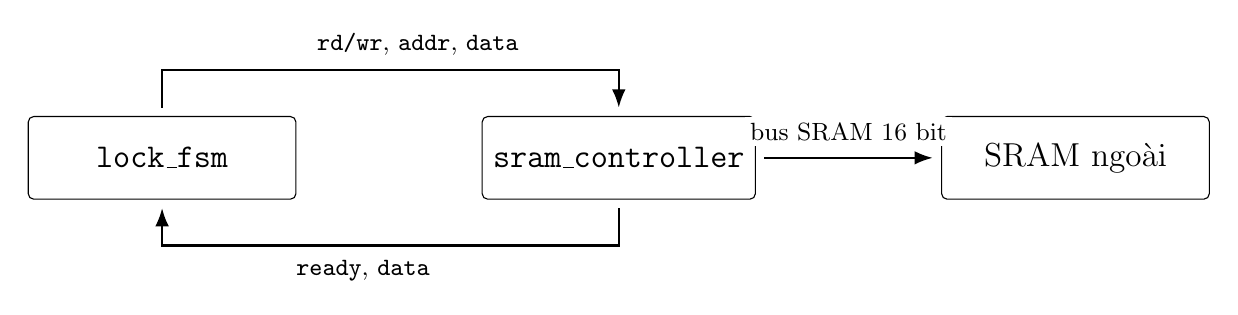
\begin{tikzpicture}[
  block/.style={draw, rounded corners=2pt, minimum width=3.4cm, minimum height=1.05cm, align=center, font=\small},
  arrow/.style={-Latex, thick, shorten >=3pt, shorten <=3pt},
  lab/.style={font=\scriptsize, fill=white, inner sep=2pt}
]
\node[block] (fsm) at (0,0) {\texttt{lock\_fsm}};
\node[block] (ctrl) at (5.8,0) {\texttt{sram\_controller}};
\node[block] (chip) at (11.6,0) {SRAM ngoài};

\draw[arrow] (fsm.north) -- ++(0,0.58) -| node[lab,pos=0.28,above=3pt]{\texttt{rd/wr}, \texttt{addr}, \texttt{data}} (ctrl.north);
\draw[arrow] (ctrl.south) -- ++(0,-0.58) -| node[lab,pos=0.28,below=3pt]{\texttt{ready}, \texttt{data}} (fsm.south);
\draw[arrow] (ctrl.east) -- node[lab,above=4pt]{bus SRAM 16 bit} (chip.west);
\end{tikzpicture}
}
\caption{Kết nối FSM với SRAM thông qua module \texttt{sram\_controller}}
\label{fig:sram}
\end{figure}

\subsection{Đọc/ghi mật khẩu}
Module \texttt{sram\_controller} quản lý bus dữ liệu hai chiều. Khi ghi, FPGA lái dữ liệu lên \texttt{SRAM\_DQ}; khi đọc, FPGA nhả bus để SRAM ngoài lái dữ liệu trả về. Đoạn mã cốt lõi có dạng:

\begin{lstlisting}[style=verilogstyle]
assign SRAM_DQ = dq_drive ? dq_out : 16'hzzzz;

// Write cycle: drive data and pull WE_N low.
dq_drive <= 1'b1;
SRAM_WE_N <= 1'b0;

// Read cycle: release data bus and pull OE_N low.
dq_drive <= 1'b0;
SRAM_OE_N <= 1'b0;
\end{lstlisting}

Sau số chu kỳ chờ được đặt bởi \texttt{SRAM\_WAIT\_CYCLES}, module đưa \texttt{o\_ready} lên mức 1 để báo cho FSM rằng thao tác đã hoàn tất.

\clearpage
\section{KẾT QUẢ TỔNG HỢP VÀ TRIỂN KHAI TRÊN QUARTUS}
\subsection{Thiết lập project}
Các thiết lập chính của project Quartus gồm:
\begin{itemize}
  \item Revision: \texttt{digital\_safe\_lock\_1}.
  \item Top-level entity: \texttt{digital\_safe\_lock}.
  \item Mã nguồn thiết kế: các file trong thư mục \texttt{design}.
  \item Bộ nhớ mật khẩu: SRAM ngoài qua module \texttt{sram\_controller}.
  \item Thiết bị đích: Cyclone IV GX \texttt{EP4CGX150DF31C7}.
\end{itemize}

\optionalimage{images/quatus.png}{Ảnh Flow Summary trong Quartus sau khi compile}{Ảnh màn hình Quartus Compile Report hoặc Project Navigator sẽ được bổ sung sau.}

\subsection{Kết quả tài nguyên}
Theo file \texttt{digital\_safe\_lock\_1.fit.summary}, quá trình Fitter thành công lúc 10:02:34 ngày 30/06/2026. Tài nguyên sử dụng được tóm tắt trong Bảng \ref{tab:resource}.

\begin{table}[H]
\centering
\caption{Tài nguyên FPGA sau tổng hợp và fitter}
\label{tab:resource}
\begin{tabular}{|l|r|}
\hline
\textbf{Chỉ tiêu} & \textbf{Kết quả}\\
\hline
Total logic elements & 349 / 149760, nhỏ hơn 1\%\\
\hline
Total combinational functions & 336 / 149760, nhỏ hơn 1\%\\
\hline
Dedicated logic registers & 187 / 149760, nhỏ hơn 1\%\\
\hline
Total registers & 187\\
\hline
Total pins & 83 / 508, 16\%\\
\hline
Total memory bits & 0 / 6635520, 0\%\\
\hline
Embedded multiplier 9-bit elements & 0 / 720, 0\%\\
\hline
Total PLLs & 0 / 8, 0\%\\
\hline
\end{tabular}
\end{table}

Kết quả trong bảng là ảnh compile cũ trước khi thêm bus SRAM vật lý. Với thiết kế mới, số chân sử dụng sẽ tăng do có thêm \texttt{SRAM\_ADDR}, \texttt{SRAM\_DQ} và các tín hiệu điều khiển SRAM. Cần chạy lại Quartus sau khi gán đúng pin SRAM trên kit để cập nhật bảng tài nguyên chính xác.

\subsection{Kết quả timing}
Timing Analyzer báo slack dương cho clock \texttt{CLOCK\_50}. Một số kết quả chính:
\begin{itemize}
  \item Slow 1200 mV 85\textdegree C setup slack: 13.507 ns.
  \item Slow 1200 mV 85\textdegree C hold slack: 0.393 ns.
  \item Slow 1200 mV 0\textdegree C setup slack: 14.030 ns.
  \item Fast 1200 mV 0\textdegree C setup slack: 16.714 ns.
  \item Fast 1200 mV 0\textdegree C hold slack: 0.175 ns.
\end{itemize}

Các slack đều dương, do đó thiết kế đáp ứng ràng buộc timing ở tần số 50 MHz trong các mô hình phân tích được Quartus báo cáo.

\subsection{Kiểm tra trên kit}
Quy trình kiểm tra phần cứng đề xuất:
\begin{enumerate}
  \item Mở project Quartus \texttt{digital\_safe\_lock\_1}.
  \item Gán đúng pin vật lý cho các tín hiệu \texttt{SRAM\_*} theo tài liệu kit hoặc Terasic System Builder.
  \item Compile và nạp file \texttt{.sof} xuống kit DE2-150.
  \item Nhấn reset bằng \texttt{KEY[0]}.
  \item Đặt \texttt{SW[7:0]=00}, nhấn \texttt{KEY[1]}, quan sát LED xanh và chữ \texttt{OPn}.
  \item Đặt \texttt{SW[7:0]=A5}, nhấn \texttt{KEY[2]}, quan sát \texttt{Chg}.
  \item Nhấn Enter để khóa lại; nhập sai \texttt{11} để kiểm tra \texttt{Err}; nhập đúng \texttt{A5} để mở lại.
  \item Nhấn reset để kiểm tra hệ thống quay về mật khẩu mặc định \texttt{00}.
\end{enumerate}

\optionalimage{images/___.png}{Ảnh thực nghiệm trạng thái khóa/chờ nhập mật khẩu}{Ảnh LED đỏ/HEX/LCD khi hệ thống chờ nhập mật khẩu sẽ được bổ sung sau.}
\optionalimage{images/open.png}{Ảnh thực nghiệm trạng thái mở khóa}{Ảnh LED xanh/HEX/LCD khi mật khẩu đúng sẽ được bổ sung sau.}
\optionalimage{images/Err.png}{Ảnh thực nghiệm trạng thái báo lỗi}{Ảnh LED đỏ/HEX/LCD khi mật khẩu sai sẽ được bổ sung sau.}
\optionalimage{images/change.png}{Ảnh thực nghiệm trạng thái đổi mật khẩu thành công}{Ảnh HEX/LCD khi đổi mật khẩu thành công sẽ được bổ sung sau.}

\clearpage
\section{KẾT LUẬN}
Dự án đã xây dựng được hệ thống khóa số bảo mật có cấu trúc RTL rõ ràng trên FPGA. Hệ thống cho phép nhập mật khẩu bằng switch, xác nhận bằng nút nhấn, mở khóa khi mật khẩu đúng, báo lỗi khi mật khẩu sai và đổi mật khẩu khi đang ở trạng thái mở khóa. Các module được tách theo chức năng: chống dội phím, FSM điều khiển, controller SRAM, LED 7 đoạn và LCD.

Thiết kế hiện tại dùng \texttt{sram\_controller} để lưu mật khẩu qua bus SRAM vật lý. Testbench đã kiểm tra thành công các luồng mở khóa, đổi mật khẩu, nhập sai và mở lại bằng mật khẩu mới với model SRAM ngoài. Bước còn lại khi chạy trên kit là gán đúng chân vật lý \texttt{SRAM\_*} trong Quartus.

\newpage
\section*{TÀI LIỆU THAM KHẢO}
\addcontentsline{toc}{section}{TÀI LIỆU THAM KHẢO}
\begin{enumerate}
  \item Intel, \textit{Quartus Prime Standard Edition Handbook}, Intel Corporation.
  \item Terasic, \textit{DE2-150 User Manual}, Terasic Technologies.
  \item Samir Palnitkar, \textit{Verilog HDL: A Guide to Digital Design and Synthesis}, Prentice Hall.
  \item Mã nguồn project khóa số bảo mật và các module Verilog đi kèm.
\end{enumerate}

\newpage
\section*{PHỤ LỤC A: MÃ NGUỒN CHÍNH}
\addcontentsline{toc}{section}{PHỤ LỤC A: MÃ NGUỒN CHÍNH}
\subsection*{A.1 Module FSM điều khiển khóa}
\lstinputlisting[style=verilogstyle]{../../design/lock_fsm.v}

\subsection*{A.2 Module điều khiển SRAM}
\lstinputlisting[style=verilogstyle]{../../design/sram_controller.v}

\subsection*{A.3 Trích đoạn testbench}
\lstinputlisting[style=verilogstyle,firstline=1,lastline=190]{../../tb/tb_digital_safe_lock.v}

\end{document}
